\begin{enumerate}[label=\thesection.\arabic*,ref=\thesection.\theenumi]
\numberwithin{equation}{enumi}
\numberwithin{figure}{enumi}
\numberwithin{table}{enumi}

	\item Find the coordinates of the focii, the vertices, the eccentricity and the length of the latus rectum of a hyperbola whose equation is given by $\frac{x^2}{16}-\frac{y^2}{9} = 1$. \\ 
		\solution
		See 
\tabref{tab:std-conic-params-sol}
and
\figref{fig:11/11/4/1Fig1}.
\begin{figure}[!h]
	\begin{center}
		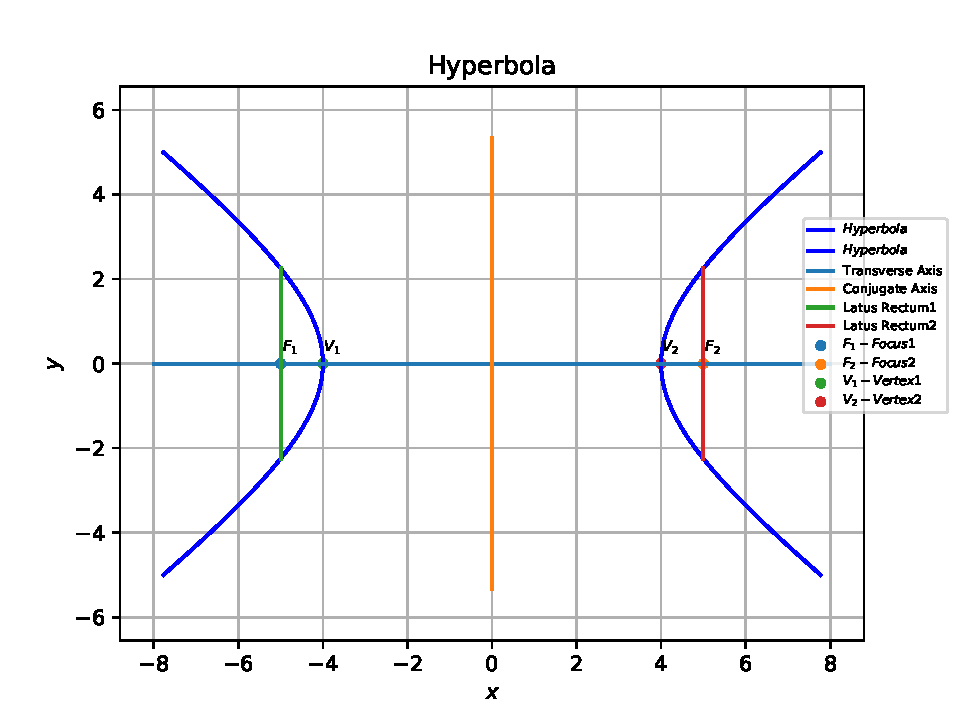
\includegraphics[width=\columnwidth]{chapters/11/11/4/1/figs/problem1.pdf}
	\end{center}
\caption{}
\label{fig:11/11/4/1Fig1}
\end{figure}

	\item Find the coordinates of the focii, the vertices, the eccentricity and the length of the latus rectum of a hyperbola whose equation is given by $\frac{y^2}{9}-\frac{x^2}{27}=1$.
		\\
		\solution
		\\
		See \tabref{tab:rot-conic-params-sol}
and 
\figref{fig:chapters/11/11/4/2/Fig1}.
\begin{figure}[H]
	\begin{center} 
	    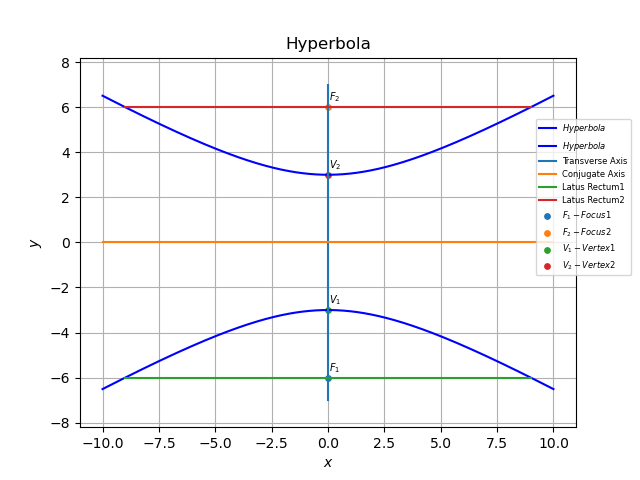
\includegraphics[width=0.75\columnwidth]{chapters/11/11/4/2/figs/hyperbola}
	\end{center}
\caption{}
\label{fig:chapters/11/11/4/2/Fig1}
\end{figure}




	\item Find the coordinates of the foci and the vertices, the eccentricity and the length of the latus rectum of the hyperbolas, whose equation is given by $5{y^2}-9{x^2}=36$.
		\\
		\solution
		\\
		\iffalse
\documentclass[journal,12pt,twocolumn]{IEEEtran}
\usepackage{setspace}
\usepackage{gensymb}
\usepackage{xcolor}
\usepackage{caption}
\singlespacing
\usepackage{siunitx}
\usepackage[cmex10]{amsmath}
\usepackage{mathtools}
\usepackage{hyperref}
\usepackage{amsthm}
\usepackage{mathrsfs}
\usepackage{txfonts}
\usepackage{stfloats}
\usepackage{cite}
\usepackage{cases}
\usepackage{subfig}
\usepackage{longtable}
\usepackage{multirow}
\usepackage{enumitem}
\usepackage{bm}
\usepackage{mathtools}
\usepackage{listings}
\usepackage{tikz}
\usetikzlibrary{shapes,arrows,positioning}
\usepackage{circuitikz}
\renewcommand{\vec}[1]{\boldsymbol{\mathbf{#1}}}
\DeclareMathOperator*{\Res}{Res}
\renewcommand\thesection{\arabic{section}}
\renewcommand\thesubsection{\thesection.\arabic{subsection}}
\renewcommand\thesubsubsection{\thesubsection.\arabic{subsubsection}}

\renewcommand\thesectiondis{\arabic{section}}
\renewcommand\thesubsectiondis{\thesectiondis.\arabic{subsection}}
\renewcommand\thesubsubsectiondis{\thesubsectiondis.\arabic{subsubsection}}
\hyphenation{op-tical net-works semi-conduc-tor}

\lstset{
language=Python,
frame=single, 
breaklines=true,
columns=fullflexible
}
\begin{document}
\theoremstyle{definition}
\newtheorem{theorem}{Theorem}[section]
\newtheorem{problem}{Problem}
\newtheorem{proposition}{Proposition}[section]
\newtheorem{lemma}{Lemma}[section]
\newtheorem{corollary}[theorem]{Corollary}
\newtheorem{example}{Example}[section]
\newtheorem{definition}{Definition}[section]
\newcommand{\BEQA}{\begin{eqnarray}}
        \newcommand{\EEQA}{\end{eqnarray}}
\newcommand{\define}{\stackrel{\triangle}{=}}
\newcommand{\myvec}[1]{\ensuremath{\begin{pmatrix}#1\end{pmatrix}}}
\newcommand{\mydet}[1]{\ensuremath{\begin{vmatrix}#1\end{vmatrix}}}
\bibliographystyle{IEEEtran}
\providecommand{\nCr}[2]{\,^{#1}C_{#2}} % nCr
\providecommand{\nPr}[2]{\,^{#1}P_{#2}} % nPr
\providecommand{\mbf}{\mathbf}
\providecommand{\pr}[1]{\ensuremath{\Pr\left(#1\right)}}
\providecommand{\qfunc}[1]{\ensuremath{Q\left(#1\right)}}
\providecommand{\sbrak}[1]{\ensuremath{{}\left[#1\right]}}
\providecommand{\lsbrak}[1]{\ensuremath{{}\left[#1\right.}}
\providecommand{\rsbrak}[1]{\ensuremath{{}\left.#1\right]}}
\providecommand{\brak}[1]{\ensuremath{\left(#1\right)}}
\providecommand{\lbrak}[1]{\ensuremath{\left(#1\right.}}
\providecommand{\rbrak}[1]{\ensuremath{\left.#1\right)}}
\providecommand{\cbrak}[1]{\ensuremath{\left\{#1\right\}}}
\providecommand{\lcbrak}[1]{\ensuremath{\left\{#1\right.}}
\providecommand{\rcbrak}[1]{\ensuremath{\left.#1\right\}}}
\theoremstyle{remark}
\newtheorem{rem}{Remark}
\newcommand{\sgn}{\mathop{\mathrm{sgn}}}
\newcommand{\rect}{\mathop{\mathrm{rect}}}
\newcommand{\sinc}{\mathop{\mathrm{sinc}}}
\providecommand{\abs}[1]{\left\vert#1\right\vert}
\providecommand{\res}[1]{\Res\displaylimits_{#1}}
\providecommand{\norm}[1]{\lVert#1\rVert}
\providecommand{\mtx}[1]{\mathbf{#1}}
\providecommand{\mean}[1]{E\left[ #1 \right]}
\providecommand{\fourier}{\overset{\mathcal{F}}{ \rightleftharpoons}}
\providecommand{\ztrans}{\overset{\mathcal{Z}}{ \rightleftharpoons}}
\providecommand{\system}[1]{\overset{\mathcal{#1}}{ \longleftrightarrow}}
\newcommand{\solution}{\noindent \textbf{Solution: }}
\providecommand{\dec}[2]{\ensuremath{\overset{#1}{\underset{#2}{\gtrless}}}}
\let\StandardTheFigure\thefigure
\def\putbox#1#2#3{\makebox[0in][l]{\makebox[#1][l]{}\raisebox{\baselineskip}[0in][0in]{\raisebox{#2}[0in][0in]{#3}}}}
\def\rightbox#1{\makebox[0in][r]{#1}}
\def\centbox#1{\makebox[0in]{#1}}
\def\topbox#1{\raisebox{-\baselineskip}[0in][0in]{#1}}
\def\midbox#1{\raisebox{-0.5\baselineskip}[0in][0in]{#1}}

\vspace{3cm}
\title{11.11.4.5}
\author{Lokesh Surana}
\maketitle
\section*{Class 11, Chapter 11, Exercise 4.5}
\fi
The equation of the hyperbola can be rearranged as
\begin{align}
	\label{eq:chapters/11/11/4/5/1}
	-x^2 + \frac{5}{9}y^2 -4 = 0
\end{align}
The above equation can be equaded to the generic equation of conic sections
\begin{align}
	\label{eq:chapters/11/11/4/5/2}
	g\brak{\vec{x}}=\vec{x}^\top \vec{V} \vec{x} + 2\vec{u}^\top \vec{x} + f = 0
\end{align}
Comparing coefficients of both equations \eqref{eq:chapters/11/11/4/5/1} and \eqref{eq:chapters/11/11/4/5/2}
\begin{align}
	\label{3}
	\vec{V} &= \myvec{-1&0\\0&\frac{5}{9}}\\
	\vec{u} &= \vec{0}\\
	f &= -4
\end{align}

From equation \eqref{3}, since $\vec{V}$ is already diagonalized, the eigen values $\lambda_1 \text{ and } \lambda_2$ are given as
\begin{align}
	\lambda_1 &= -1\\
	\lambda_2 &= \frac{5}{9}
\end{align}
\begin{enumerate}
\item The eccentricity of the hyperbola is given as
\begin{align}
	e &= \sqrt{1 - \frac{\lambda_2}{\lambda_1}} = \sqrt{1+\frac{5}{9}}\\
	  &= \frac{\sqrt{14}}{3}
\end{align}
\item For the standard hyperbola, the coordinates of Focii are given as
\begin{align}
	\label{eq:chapters/11/11/4/5/4}
	\vec{F} = \pm \frac{\brak{\frac{1}{e\sqrt{1-e^2}}}\brak{e^2}\sqrt{\frac{\lambda_1}{f_0}}}{\frac{\lambda_1}{f_0}} \vec{e}_2
\end{align}
where
\begin{align}
	f_0 &= -f\\
	\eqref{eq:chapters/11/11/4/5/4} \implies &= \pm \frac{\brak{\frac{1}{\frac{\sqrt{14}}{3}\sqrt{1-\frac{14}{9}}}}\brak{\frac{14}{9}}\sqrt{\frac{-1}{4}}}{\frac{-1}{4}} \vec{e}_2\\
	&= \pm \myvec{0\\\frac{6}{2\sqrt{\frac{14}{5}}}}
\end{align}
\item The vertices of the hyperbola are given by
\begin{align}
	\pm \myvec{0\\\sqrt{\abs{\frac{f_0}{\lambda_2}}}}= \pm \myvec{0\\\frac{6}{\sqrt{5}}}
\end{align}
\item The length of latus rectum is given as
\begin{align}
	2\frac{\sqrt{\abs{f_0 \lambda_2}}}{\lambda_1} &= 2\frac{\sqrt{\abs{14\brak{\frac{5}{9}}}}}{-1}\\
	&= 4\frac{\sqrt{5}}{3}
\end{align}
as length cannot be negative.
\end{enumerate}

\begin{figure}[!h]
	\begin{center} 
	    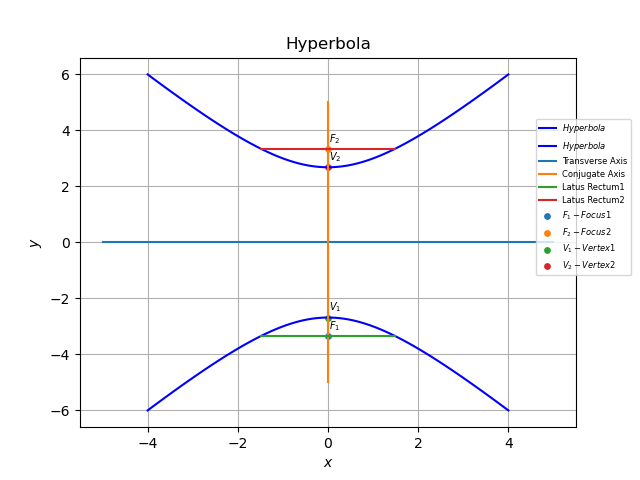
\includegraphics[width=\columnwidth]{chapters/11/11/4/5/figs/hyperbola.png}
	\end{center}
\caption{}
\label{fig:chapters/11/11/4/5/1}
\end{figure}


	\item Find the equation of the hyperbola whose foci is $\brak{0,\pm 8}$ and vertices $\brak{0,\pm 5}$.
\\
\solution
\item Find the equations of hyperbola having Vertices $\myvec{0\\\pm 3}$ and Foci $\myvec{0\\\pm5}$
	\\
\solution
		\iffalse
\documentclass[journal,12pt,twocolumn]{IEEEtran}
%
\usepackage{setspace}
\usepackage{gensymb}
%\doublespacing
\singlespacing

%\usepackage{graphicx}
%\usepackage{amssymb}
%\usepackage{relsize}
\usepackage[cmex10]{amsmath}
%\usepackage{amsthm}
%\interdisplaylinepenalty=2500
%\savesymbol{iint}
%\usepackage{txfonts}
%\restoresymbol{TXF}{iint}
%\usepackage{wasysym}
\usepackage{amsthm}
%\usepackage{iithtlc}
\usepackage{mathrsfs}
\usepackage{txfonts}
\usepackage{stfloats}
\usepackage{bm}
\usepackage{cite}
\usepackage{cases}
\usepackage{subfig}
%\usepackage{xtab}
\usepackage{longtable}
\usepackage{multirow}
%\usepackage{algorithm}
%\usepackage{algpseudocode}
\usepackage{enumitem}
\usepackage{mathtools}
\usepackage{steinmetz}
\usepackage{tikz}
\usepackage{circuitikz}
\usepackage{verbatim}
\usepackage{tfrupee}
\usepackage[breaklinks=true]{hyperref}
%\usepackage{stmaryrd}
\usepackage{tkz-euclide} % loads  TikZ and tkz-base
%\usetkzobj{all}
\usetikzlibrary{calc,math}
\usepackage{listings}
    \usepackage{color}                                            %%
    \usepackage{array}                                            %%
    \usepackage{longtable}                                        %%
    \usepackage{calc}                                             %%
    \usepackage{multirow}                                         %%
    \usepackage{hhline}                                           %%
    \usepackage{ifthen}                                           %%
  %optionally (for landscape tables embedded in another document): %%
    \usepackage{lscape}     
\usepackage{multicol}
\usepackage{chngcntr}
%\usepackage{enumerate}

%\usepackage{wasysym}
%\newcounter{MYtempeqncnt}
\DeclareMathOperator*{\Res}{Res}
%\renewcommand{\baselinestretch}{2}
\renewcommand\thesection{\arabic{section}}
\renewcommand\thesubsection{\thesection.\arabic{subsection}}
\renewcommand\thesubsubsection{\thesubsection.\arabic{subsubsection}}

\renewcommand\thesectiondis{\arabic{section}}
\renewcommand\thesubsectiondis{\thesectiondis.\arabic{subsection}}
\renewcommand\thesubsubsectiondis{\thesubsectiondis.\arabic{subsubsection}}

% correct bad hyphenation here
\hyphenation{op-tical net-works semi-conduc-tor}
\def\inputGnumericTable{}                                 %%

\lstset{
%language=C,
frame=single, 
breaklines=true,
columns=fullflexible
}
%\lstset{
%language=tex,
%frame=single, 
%breaklines=true
%}

\begin{document}
%


\newtheorem{theorem}{Theorem}[section]
\newtheorem{problem}{Problem}
\newtheorem{proposition}{Proposition}[section]
\newtheorem{lemma}{Lemma}[section]
\newtheorem{corollary}[theorem]{Corollary}
\newtheorem{example}{Example}[section]
\newtheorem{definition}[problem]{Definition}
%\newtheorem{thm}{Theorem}[section] 
%\newtheorem{defn}[thm]{Definition}
%\newtheorem{algorithm}{Algorithm}[section]
%\newtheorem{cor}{Corollary}
\newcommand{\BEQA}{\begin{eqnarray}}
\newcommand{\EEQA}{\end{eqnarray}}
\newcommand{\define}{\stackrel{\triangle}{=}}

\bibliographystyle{IEEEtran}
%\bibliographystyle{ieeetr}


\providecommand{\mbf}{\mathbf}
\providecommand{\pr}[1]{\ensuremath{\Pr\left(#1\right)}}
\providecommand{\qfunc}[1]{\ensuremath{Q\left(#1\right)}}
\providecommand{\sbrak}[1]{\ensuremath{{}\left[#1\right]}}
\providecommand{\lsbrak}[1]{\ensuremath{{}\left[#1\right.}}
\providecommand{\rsbrak}[1]{\ensuremath{{}\left.#1\right]}}
\providecommand{\brak}[1]{\ensuremath{\left(#1\right)}}
\providecommand{\lbrak}[1]{\ensuremath{\left(#1\right.}}
\providecommand{\rbrak}[1]{\ensuremath{\left.#1\right)}}
\providecommand{\cbrak}[1]{\ensuremath{\left\{#1\right\}}}
\providecommand{\lcbrak}[1]{\ensuremath{\left\{#1\right.}}
\providecommand{\rcbrak}[1]{\ensuremath{\left.#1\right\}}}
\theoremstyle{remark}
\newtheorem{rem}{Remark}
\newcommand{\sgn}{\mathop{\mathrm{sgn}}}
\providecommand{\abs}[1]{\left\vert#1\right\vert}
\providecommand{\res}[1]{\Res\displaylimits_{#1}} 
\providecommand{\norm}[1]{\left\lVert#1\right\rVert}
%\providecommand{\norm}[1]{\lVert#1\rVert}
\providecommand{\mtx}[1]{\mathbf{#1}}
\providecommand{\mean}[1]{E\left[ #1 \right]}
\providecommand{\fourier}{\overset{\mathcal{F}}{ \rightleftharpoons}}
%\providecommand{\hilbert}{\overset{\mathcal{H}}{ \rightleftharpoons}}
\providecommand{\system}{\overset{\mathcal{H}}{ \longleftrightarrow}}
	%\newcommand{\solution}[2]{\textbf{Solution:}{#1}}
\newcommand{\solution}{\noindent \textbf{Solution: }}
\newcommand{\cosec}{\,\text{cosec}\,}
\providecommand{\dec}[2]{\ensuremath{\overset{#1}{\underset{#2}{\gtrless}}}}
\newcommand{\myvec}[1]{\ensuremath{\begin{pmatrix}#1\end{pmatrix}}}
\newcommand{\mydet}[1]{\ensuremath{\begin{vmatrix}#1\end{vmatrix}}}
%\numberwithin{equation}{section}
\numberwithin{equation}{subsection}
%\numberwithin{problem}{section}
%\numberwithin{definition}{section}
\makeatletter
\@addtoreset{figure}{problem}
\makeatother

\let\StandardTheFigure\thefigure
\let\vec\mathbf
%\renewcommand{\thefigure}{\theproblem.\arabic{figure}}
\renewcommand{\thefigure}{\theproblem}
%\setlist[enumerate,1]{before=\renewcommand\theequation{\theenumi.\arabic{equation}}
%\counterwithin{equation}{enumi}


%\renewcommand{\theequation}{\arabic{subsection}.\arabic{equation}}

\def\putbox#1#2#3{\makebox[0in][l]{\makebox[#1][l]{}\raisebox{\baselineskip}[0in][0in]{\raisebox{#2}[0in][0in]{#3}}}}
     \def\rightbox#1{\makebox[0in][r]{#1}}
     \def\centbox#1{\makebox[0in]{#1}}
     \def\topbox#1{\raisebox{-\baselineskip}[0in][0in]{#1}}
     \def\midbox#1{\raisebox{-0.5\baselineskip}[0in][0in]{#1}}

\vspace{3cm}


\title{Que: 11.11.4.9}
\author{Nikam Pratik Balasaheb (EE21BTECH11037)}





% make the title area
\maketitle

\newpage

%\tableofcontents

\bigskip

\renewcommand{\thefigure}{\theenumi}
\renewcommand{\thetable}{\theenumi}
%\renewcommand{\theequation}{\theenumi}

\section{Problem}

\section{Solution}
\fi

\begin{enumerate}

	\item Transverse axis:
Line joining two foci
\begin{align}
	\vec{m} &= \vec{F}_1 - \vec{F}_2\\
	&= \myvec{0 \\ 10}\\
	\myvec{1&0}\brak{\vec{x} -\vec{F}_1} &= 0\\
	\myvec{1& 0}\vec{x} &= 0
\end{align}

\item Center of hyperbola, $\vec{O}$ is given by:
\begin{align}
	\vec{O} &= \frac{\vec{F}_1 + \vec{F}_2}{2}\\
	\vec{O} &= \myvec{0\\0}
\end{align}

\item Normal vector of directrix
	\begin{align}
		\vec{n} &= \text{direction vector of transverse axis}\\
			&= \myvec{0 \\1}
	\end{align}
%
\begin{align}
	\vec{V} &= \norm{\vec{n}}^2\vec{I} - e^2\vec{n}\vec{n}^{\top}\\
		&= \myvec{1 & 0 \\ 0 & 1} - e^2\myvec{ 0 & 0 \\ 0 & 1}\\
		&= \myvec{1 &0\\ 0 & 1-e^2}
\end{align}
%
\begin{align}
	\vec{u} &= ce^2\vec{n} -\norm{\vec{n}}^2\vec{F}\\
		&= \myvec{0\\ ce^2 - 5}
\end{align}
%
\begin{align}
	f &= \norm{\vec{n}}^2\norm{\vec{F}}^2 - c^2e^2\\
	  &= 25 - c^2 e^2
\end{align}
%
Equation of the hyperbola
\begin{align}
	\vec{x}^{\top}\vec{V}\vec{x} +2\vec{u}^{\top}\vec{x}+f &= 0
\end{align}
%
Vertex lies on this curve,
\begin{align}
	\vec{v_1}^{\top}\vec{V}\vec{v_1} +2\vec{u}^{\top}\vec{v_1}+f &= 0\\
	9\brak{1-e^2} + 6 \brak{ce^2 -5} - c^2e^2 +25 &= 0\\
	4 -9e^2 +6ce^2 -c^2e^2 &= 0 \label{eq:chapters/11/11/4/9/1}
\end{align}
Also, the center is given by,
\begin{align}
	\vec{O} &= - \vec{V}^{-1} \vec{u}\\
	\myvec{0\\0} &= \myvec{0\\ \frac{ce^2-5}{1-e^2}}\\
	ce^2 &= 5
	\label{eq:chapters/11/11/4/9/2}
\end{align}
%
Solving \eqref{eq:chapters/11/11/4/9/1} and \eqref{eq:chapters/11/11/4/9/2},
\begin{align}
	c &= \frac{9}{5} \\
	e &= \frac{5}{3}
\end{align}
%
\begin{align}
	\vec{V} &= \myvec{1&0\\0& -\frac{16}{9}} \\
	\vec{u} &= \myvec{0\\0}\\
	f &= 16
\end{align}
%
Equation of the Hyperbola,
\begin{align}
	\vec{x}^{\top} \myvec{1&0\\ 0 & -\frac{16}{9}} \vec{x} +16 =0
\end{align}
%
\begin{table}[h!]
	\begin{center}
	%%%%%%%%%%%%%%%%%%%%%%%%%%%%%%%%%%%%%%%%%%%%%%%%%%%%%%%%%%%%%%%%%%%%%%
%%                                                                  %%
%%  This is a LaTeX2e table fragment exported from Gnumeric.        %%
%%                                                                  %%
%%%%%%%%%%%%%%%%%%%%%%%%%%%%%%%%%%%%%%%%%%%%%%%%%%%%%%%%%%%%%%%%%%%%%%

\begin{tabular}[]{|c|c|c|}
\hline
Parameter & Value & Description \\ \hline
$\vec{F}_1$	& $\myvec{0\\5}$ & Focus\\ \hline
$\vec{F}_2$	& $\myvec{0\\-5}$ & Focus\\ \hline
$\vec{v}_1$	& $\myvec{0\\3}$ & Vertex \\ \hline
$\vec{v}_2$ 	& $\myvec{0\\-3}$ & Vertex\\ \hline
\end{tabular}

\end{center}
\caption{}
\label{tab:chapters/11/11/4/9/}
\end{table}
%
\begin{figure}[h!]
  \centering
    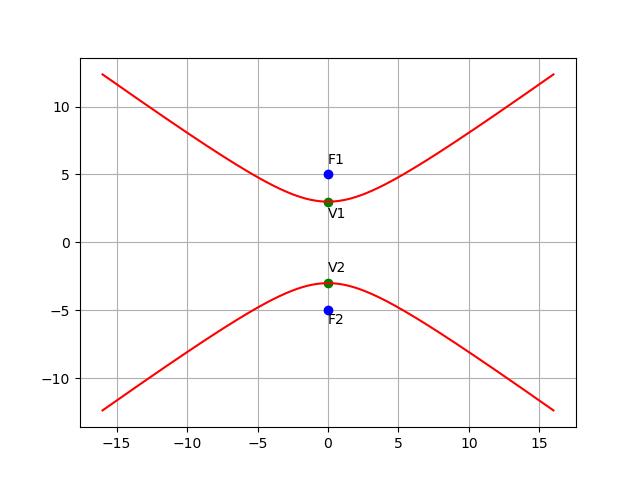
\includegraphics[width=\columnwidth]{chapters/11/11/4/9/figs/Figure_1.png}
    \caption{Figure 1}
    \label{fig:chapters/11/11/4/9/}
\end{figure}
%
\end{enumerate}




	It is obvious that
	\begin{align}
		\vec{n} 
			= \vec{e}_2,
	\vec{c} =\vec{u}=\vec{0}.
\end{align}
Consequently,
%
\begin{align}
	\vec{V} &= \myvec{1 &0\\ 0 & 1-e^2}
	\\
	\vec{F} &= ce^2\vec{e}_2 \implies \norm{\vec{F}} = ce^2=8
\label{eq:chapters/11/11/4/8/F}
	\\
	f 
	  &= 64 - c^2 e^2
\label{eq:chapters/11/11/4/8/f}
\end{align}
%
Since the vertices are  on the conic,
\begin{align}
	\vec{v_1}^{\top}\vec{V}\vec{v_1} +2\vec{u}^{\top}\vec{v_1}+f &= 0\\
\implies 25\brak{1-e^2} + f &= 0\\
	 \label{eq:chapters/11/11/4/8/1}
\end{align}
Solving \eqref{eq:chapters/11/11/4/8/1},
\eqref{eq:chapters/11/11/4/8/F}
and
\eqref{eq:chapters/11/11/4/8/f},
\begin{align}
	c = \frac{9}{5},\ 
	e = \frac{5}{3},
\end{align}
%
yielding
\begin{align}
	\vec{V} = \myvec{1&0\\0& -\frac{16}{9}} ,\
	\vec{u} = \myvec{0\\0},\
	f = 16.
\end{align}
%
Thus, the desired equation of the hyperbola is
\begin{align}
	\vec{x}^{\top} \myvec{1&0\\ 0 & -\frac{16}{9}} \vec{x} +16 =0
\end{align}
%
\item We know the Focii is given as
\begin{align}
	\vec{F} &= \pm \frac{\brak{\frac{1}{e\sqrt{1-e^2}}}\brak{e^2}\sqrt{\frac{\lambda_1}{f_0}}}{\frac{\lambda_1}{f_0}}\vec{e}_2\\
	        &= \frac{\frac{e}{\sqrt{1-e^2}}}{\sqrt{\frac{\lambda_1}{f_0}}}\vec{e}_2
\end{align}
Substituting \eqref{eq:chapters/11/11/4/8/eq1} we get
\begin{align}
	\vec{F} &= 5e\vec{e}_2\\
	\myvec{0\\8} &= 5e\vec{e}_2\\
	\implies e &= \frac{8}{5}
\end{align}
\item Now we know the eccentricity is given as
\begin{align}
	e = \sqrt{1-\frac{\lambda_2}{\lambda_1}}\\
	\label{eq:chapters/11/11/4/8/eq2}
	\implies \frac{\lambda_2}{\lambda_1} = -\frac{39}{25}
\end{align}
\item Now we know from the standard equation
\begin{align}
	\label{eq:chapters/11/11/4/8/eq3}
	f = \norm{\vec{n}}^2 \norm{\vec{F}}^2 - c^2 e^2
\end{align}
Calculating $\vec{n} \text{ and } c$
\begin{align}
	\vec{n} &= \sqrt{\frac{\lambda_1}{f_0}}\vec{e}_2 = \frac{1}{5}\sqrt{\frac{\lambda_1}{\lambda_2}}\vec{e}_2\\
	        &= \frac{1}{\sqrt{-39}}\vec{e}_2\\
	c &= \frac{1}{e\sqrt{1-e^2}} = \frac{25}{8\sqrt{-39}}	
\end{align}
Now
\begin{align}
	\norm{\vec{n}}^2 &= -\frac{1}{39}\\
	\norm{\vec{F}}^2 &= 64
\end{align}
Substituting all the values in \eqref{eq:chapters/11/11/4/8/eq3} we get
\begin{align}
	f &= -\brak{\frac{1}{39}}\brak{64} + \brak{\frac{25}{8}}^2 \brak{\frac{1}{39}} \brak{\frac{64}{25}}\\
	  &= -1\\
	\label{eq:chapters/11/11/4/8/eq4}  
	f_0  &= -f = 1
\end{align}
substituting \eqref{eq:chapters/11/11/4/8/eq4} in \eqref{eq:chapters/11/11/4/8/eq1} we get
\begin{align}
	\label{eq:chapters/11/11/4/8/eq5}
	\lambda_2 = \frac{1}{25} 
\end{align}
Substituting \eqref{eq:chapters/11/11/4/8/eq5} in \eqref{eq:chapters/11/11/4/8/eq2} we get
\begin{align}
	\lambda_1 = -\frac{1}{39}
\end{align}
\end{enumerate}
Therefore the equation of the hyperbola is given as
\begin{align}
	g\brak{\vec{x}}=\vec{x}^\top \vec{V} \vec{x} + 2\vec{u}^\top \vec{x} + f = 0
\end{align}
where
\begin{align}
	\vec{V} &= \myvec{\lambda_1&0\\0&\lambda_2} = \myvec{-\frac{1}{39}&0\\0&\frac{1}{25}}\\
	\vec{u} &= \vec{0}\\
	f &= -1
\end{align}
See Fig. \ref{fig:chapters/11/11/4/8/Fig1}.
\begin{figure}[H]
	\begin{center} 
	    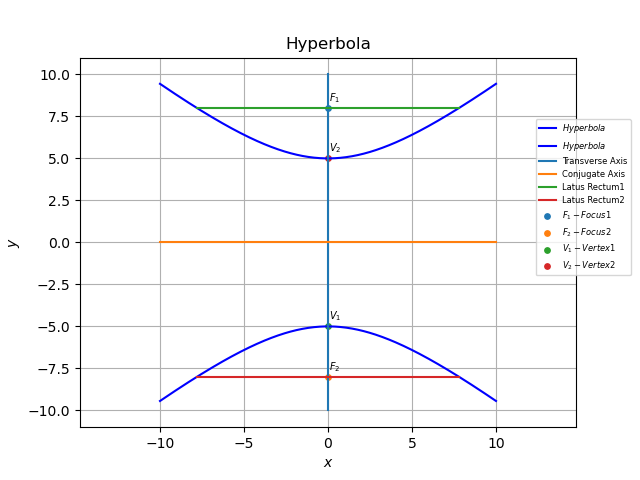
\includegraphics[width=0.75\columnwidth]{chapters/11/11/4/8/figs/hyperbola2}
	\end{center}
\caption{}
\label{fig:chapters/11/11/4/8/Fig1}
\end{figure}


\item Find the equation of the hyperbola that satisfies the conditions - Foci \brak{\pm 4, 0}, the latus rectum is of length 12.
\\
\solution
		The given information is available in 
\tabref{tab:chapters/11/11/4/13/1}.
Since two foci are given, the conic cannot be a parabola.
The equation of the conic with focus $\vec{F}$, directrix $\vec{n}^\top\vec{x} = c$ and eccentricity $e$ is given by
\begin{align}
\vec{V} &\triangleq \norm{\vec{n}}^2\vec{I} - e^2\vec{n}\vec{n}^\top \label{eq:chapters/11/11/4/13/2} \\
\vec{u} &\triangleq ce^2\vec{n} - \norm{\vec{n}}^2\vec{F} \label{eq:chapters/11/11/4/13/3} \\
f &\triangleq \norm{\vec{n}}^2\norm{\vec{F}}^2 - c^2e^2 \label{eq:chapters/11/11/4/13/4}
\end{align}
also
\begin{align}
f_0 &= \vec{u}^\top\vec{V}^{-1}\vec{u} - f\\
l &= 2\frac{\sqrt{\abs{f_0\lambda_2}}}{\lambda_1}
\end{align}

\begin{enumerate}
\item The direction vector of $F_1F_2$ is the normal vector of the directrix.  Hence, 
\begin{align}
\vec{n} = \vec{F_1} - \vec{F_2}
	\equiv \vec{e}_1
\end{align}
Substituting in 
  \eqref{eq:conic_quad_form_v},
\eqref{eq:conic_quad_form_u}
and
\eqref{eq:conic_quad_form_f},
\begin{align}
	\vec{V} &= \myvec{1-e^2&0\\0&1} \label{eq:chapters/11/11/4/13/6} 
	\\
	\vec{u} &= ce^2\vec{e}_1-\vec{F}
\label{eq:chapters/11/11/4/13/6/u} 
	\\
	f&=16-c^2e^2
\label{eq:chapters/11/11/4/13/6/f} 
\end{align}
\item From
\eqref{eq:chapters/11/11/4/13/6},
\begin{align}
\lambda_1 &= 1-e^2,\
\lambda_2 = 1
\label{eq:chapters/11/11/4/13/12}
\end{align}
which upon substituting
in
			\eqref{eq:latus-ellipse}, along with the value of the latus rectum 
from \tabref{tab:chapters/11/11/4/13/1}
		\begin{align}
	6\brak{1-e^2} = \sqrt{\abs{f}}
\label{eq:chapters/11/11/4/13/12/f}
\end{align}
\item  The centre of the conic is given by
\begin{align}
\vec{c} = \frac{\vec{F_1} + \vec{F_2}}{2}
= \vec{0}
\label{eq:chapters/11/11/4/13/5}
\end{align}
From \eqref{eq:chapters/11/11/4/13/6}, it is obvious that  
$\vec{V}$ is invertible.  Hence,  
from \eqref{eq:chapters/11/11/4/13/5}
and 
\eqref{eq:conic_parmas_c_def},
\begin{align}
\vec{u} = \vec{0}
	\label{eq:chapters/11/11/4/13/7/u}
\end{align}
Substituting the above in \eqref{eq:chapters/11/11/4/13/6/u}, 
\begin{align}
\vec{F} = ce^2\vec{e}_1 
\implies 
	\norm{\vec{F}} = 4 = ce^2
	\label{eq:chapters/11/11/4/13/7}
\end{align}
\item 
	From 
      \eqref{eq:f0}, 
	\eqref{eq:chapters/11/11/4/13/7/u}
and
\eqref{eq:chapters/11/11/4/13/6/f},
		\begin{align}
	36\brak{1-e^2}^2 = 16-c^2e^2
\label{eq:chapters/11/11/4/13/12/ec}
\end{align}
From
	\eqref{eq:chapters/11/11/4/13/7}
	and
\eqref{eq:chapters/11/11/4/13/12/ec}
\begin{align}
\frac{4}{e\sqrt{e^2-1}} &= 6
\\
\implies 9e^2\brak{e^2-1} &= 4\\
\implies 9e^4-9e^2-4 &= 0
\\
	\text{or, }\brak{3e^2-4}
	\brak{12e^2+1} &=0
\label{eq:chapters/11/11/4/13/14}
\end{align}
yielding
\begin{align}
e = \frac{4}{3}
\end{align}
as the only viable solution.
\end{enumerate}
The equation of the conic is then obtained as
\begin{align}
\vec{x}^\top\myvec{-\frac{1}{3}&0\\0&1}\vec{x} +4 = 0
\end{align}
See \figref{fig:chapters/11/11/4/13/1}.
\begin{figure}[ht]
\centering
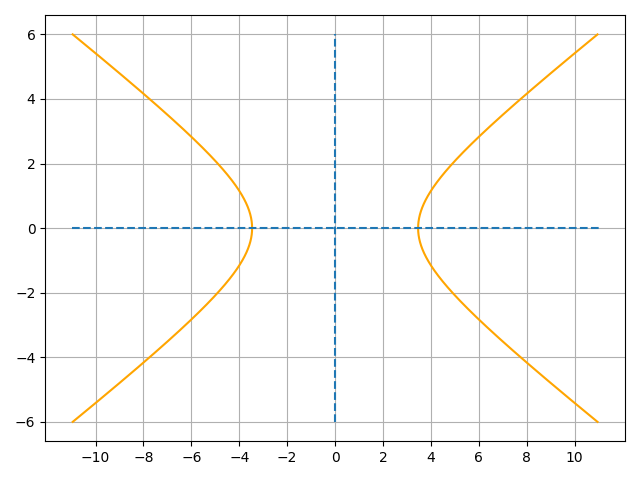
\includegraphics[width = \columnwidth]{chapters/11/11/4/13/figs/fig1.png}
\caption{}
\label{fig:chapters/11/11/4/13/1}
\end{figure}
\begin{table}[h]
\centering
%%%%%%%%%%%%%%%%%%%%%%%%%%%%%%%%%%%%%%%%%%%%%%%%%%%%%%%%%%%%%%%%%%%%%%
%%                                                                  %%
%%  This is a LaTeX2e table fragment exported from Gnumeric.        %%
%%                                                                  %%
%%%%%%%%%%%%%%%%%%%%%%%%%%%%%%%%%%%%%%%%%%%%%%%%%%%%%%%%%%%%%%%%%%%%%%

\begin{center}
\begin{tabular}{|c|c|c|}
\hline
\textbf{Parameter}& \textbf{Description} &\textbf{Value}\\ \hline
$\vec{F_1}$		 &	Focus 1 of hyperbola&$\myvec{4\\0}$\\ \hline
$\vec{F_2}$		 &	Focus 2 of hyperbola&$\myvec{-4\\0}$\\ \hline
$l$		 &  Length of latus rectum&12 \\ \hline
\end{tabular}
\end{center}

\caption{}
\label{tab:chapters/11/11/4/13/1}
\end{table}

    \item Find the equation of the hyperbola whose eccentricity is $e = \frac{4}{3}$
    and whose vertices are
    \begin{align}
        \vec{P_1} = \myvec{7\\0},\ \vec{P_2} = \myvec{-7\\0}
        \label{eq:chapters/11/11/4/14/vert}
    \end{align}
\\
\solution
		    The major axis of a conic is the chord which passes through the vertices of the conic.
    The direction vector of the major axis in this case is
    \begin{align}
        \vec{P}_2-\vec{P}_1 \equiv \vec{e}_1 = \vec{n}
\label{eq:chapters/11/11/4/13/6/n} 
    \end{align}
    which is the normal vector for the directrix.
    Since $e > 1$, the conic is a hyperbola.
Substituting  
\eqref{eq:chapters/11/11/4/13/6/n} 
in
  \eqref{eq:conic_quad_form_v},
\eqref{eq:conic_quad_form_u}
and
\eqref{eq:conic_quad_form_f},
\begin{align}
	\vec{V} &= \myvec{1-e^2&0\\0&1} = \myvec{-\frac{7}{9}&0\\0&1} \label{eq:chapters/11/11/4/14/6} 
	\\
	\vec{u} &= ce^2\vec{e}_1-\vec{F}
\label{eq:chapters/11/11/4/14/6/u} 
	\\
	f&=16-c^2e^2
\label{eq:chapters/11/11/4/14/6/f} 
\end{align}
    Thus,
    \begin{align}
        \vec{V} = \myvec{1-e^2&0\\0&1} \label{eq:chapters/11/11/4/14/V-val} \\
	    \vec{u} = ce^2\vec{e}_1 - \vec{F} \label{eq:chapters/11/11/4/14/u-val} \\
        f = \norm{\vec{F}}^2 - c^2e^2 \label{eq:chapters/11/11/4/14/f-val}
    \end{align}
    The centre of the hyperbola is 
\begin{align}
	\vec{c} = \frac{\vec{P}_1+\vec{P}_2}{2} = \vec{0} = \vec{u}
\end{align}
from \eqref{eq:conic_parmas_c_def}.      Substituting $\vec{P}_1$ and $\vec{P}_2$ in 
    \eqref{eq:conic_quad_form},
    \begin{align}
        \vec{P}_1^\top\vec{VP}_1 + 2\vec{u}^\top\vec{P}_1 + f &= 0 \label{eq:chapters/11/11/4/14/ep1} \\
        \vec{P}_2^\top\vec{VP}_2 + 2\vec{u}^\top\vec{P}_2 + f &= 0 \label{eq:chapters/11/11/4/14/ep2}
	\\
	    \implies f = \vec{P}_1^\top\vec{VP}_1  = 49\brak{e^2-1}&=\frac{343}{9}
    \end{align}
    upon adding 
    \eqref{eq:chapters/11/11/4/14/ep2} and \eqref{eq:chapters/11/11/4/14/ep1}
    and simplifying.
    Therefore, the equation of the conic is
    \begin{align}
        \vec{x}^\top\myvec{-\frac{7}{9}&0\\0&1}\vec{x} + \frac{343}{9} = 0
    \end{align}
See \figref{fig:chapters/11/11/4/14/hyperbola}.
    \begin{figure}[!ht]
        \centering
        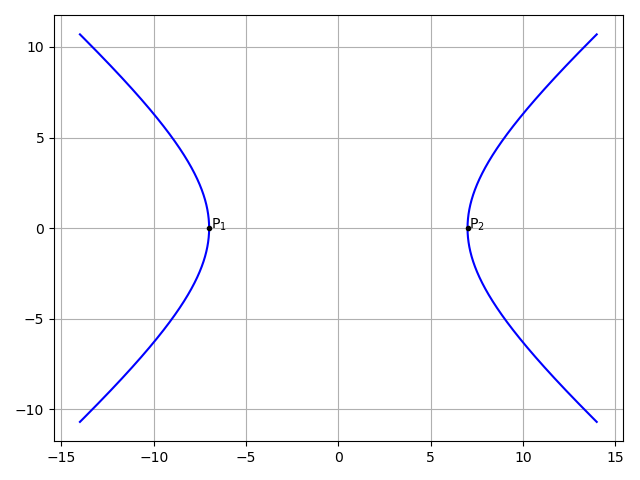
\includegraphics[width=\columnwidth]{chapters/11/11/4/14/figs/hyperbola.png}
        \caption{}
        \label{fig:chapters/11/11/4/14/hyperbola}
    \end{figure}


\end{enumerate}
